\section{Construccionismo y las TIC}

El construccionismo es una corriente pedagógica con un enfoque diferente en
cuanto al uso de las TIC en la educación. Esta pedagogía se diferencia de la
educación tradicional en que el estudiante ya no es un receptor pasivo de
información, en cambio, el mismo participa activamente del proceso de
aprendizaje construyendo su propio conocimiento. 

El construccionismo utiliza la tecnología como medio cognitivo  a diferencia de
la educación tradicional que la utiliza para la entrega de contenido. 

El construccionismo es un alternativa prometedora a la educación
tradicional.Desde el punto de vista tecnológico, el contruccionismo es ideal
pues el mismo requiere un alto dinamismo en el traspaso del conocimiento
\cite{sasha:construtivism}. 

El contruccionismo y las \Gls{tic} siempre han estado relacionados, ya que el
mismo se originó con un lenguaje de programación(LOGO)\cite{ict:ttc}. Un
característica importante de esta relación es que tienen la capacidad de
eliminar los problemas de distancia\cite{mariluz:seiousgames}.


\subsection{Historia}

Seymour Papert adoptó el término construccionismo en la década de 1980 para
representar una método pedagógico practicado por John Dewey a principios del
siglo 20. Este método buscaba que la responsabilidad de aprender recaiga en el
estudiante. 

Papert trabajó directamente con el psicólogo evolutivo y filósofo suizo Jean
Piaget. Este último, había elaborado con anterioridad sus teorías de la
educación y construcción del conocimiento al ver e interactuar con los niños y a
partir de esta observación dio origen al constructivismo, según el cual, el
conocimiento debe ser construido por el estudiante y los nuevos significados
deben ser obtenidos relacionándolos con significados anteriores por los mismos
estudiantes haciendo uso así de sus propios sistemas de relaciones.

El construccionismo se diferencia de lo anterior en que los estudiantes
construyen las ideas o partes del mundo utilizando herramientas. La elaboración
de representaciones mentales mediante la construcción y el intercambio es la
metáfora del marco contruccionista. 

Durante 1980, Seymor Papert, Wally Feurzeig, Marvin Minsky y John McCarthy y los
miembros del Departamento de Inteligencia Artificial del \Gls{mit} y una
compañía de tecnología en Cambridge, Massachusetts, desarrollaron un nuevo
lenguaje de programación llamado LOGO que tenía por objeto que los estudiantes
construyeran sus modelos en notación LOGO\@. Este juego introduciría de forma
natural las ideas de los procedimientos, funciones, variables, recursividad, la
modularidad, simulación, verificación, entre otros.

La creación del lenguaje de programación LOGO dio inicio al construccionismo.

Los desarrolladores de LOGO no solo alentaron la promoción de formas
construccionistas de enseñanza y aprendizaje sino también alentaron otra forma
de aprendizaje nueva y no tradicional diferentes a las tradicionales si no
también alentaron otra forma de aprendizaje nueva y no tradicional con las
herramientas tecnológicas. 

De vuelta en la década de 1980, cuando se produjo LOGO y se acuñó el
construccionismo, la comunidad del contruccionismo era en su mayoría  ingenieros
informáticos y matemáticos \cite{historia:2014}.

\subsection{Bases Pedagógicas}

Para el construccionismo, el conocimiento es construido por el estudiante en
lugar de ser trasmitido por el profesor\cite{moses:2003} y esto sucede
particularmente cuando el mismo se compromete en la elaboración de un producto o
artefacto que tenga un significado y pueda ser compartido\cite{valdivia:sg}. De
esta manera, se permite a los estudiantes elaborar sus propias interpretaciones
razonadas del mundo mediante la interacción con el mismo.

Según Papert, los alumnos estarán mucho más involucrados en su aprendizaje si
construyen artefactos que los demás pueden ver, criticar y tal vez utilizar. Y
además, el alumno se enfrenta a problemas complejos con estas construcciones,
harán el esfuerzo por resolver problemas y aprender ya que la construcción les
motivará\cite{const:vs}.

El enfoque construccionista establece que los seres humanos conocen y aprenden
de formas diferentes por lo tanto, no se puede elaborar una jerarquía de estilos
de aprendizajes\cite{valdivia:sg}.

\subsection{Estado del Arte}

El construccionismo pone énfasis en el \emph{Aprender haciendo}, esta idea
mejora la práctica educativa tradicional o instruccionismo. El instruccionismo
se basa en el concepto de que existe un profesor y un estudiante, el profesor
transfiere el conocimiento que ha adquirido a un alumno que es receptor pasivo
de información de esta manera, se enfoca más en la capacidad del profesor. 

Existen varios emprendimientos o \emph{amigos del contruccionismo}, para la
mayoría de ellos las computadoras son esenciales mientras que para otros el
mayor esfuerzo está en la incorporación de la tecnología en su práctica
educativa~\cite{papertian:const}.

Algunos de estos emprendimientos son:

\begin{description}

\item[Lenguaje de programación LOGO]  A mediados de la década de 1960 Seymour
	Papert, que había estado trabajando con Piaget en Ginebra, llegó a
	Estados Unidos donde co-fundó el Laboratorio de Inteligencia Artifical
	del MIT con Marvin Minsky. Papert trabajó con el equipo de Bolt, Beranek
	y Newman, liderado por Wallace Feurzeig, que creó la primera versión del
	logotipo en 1967. A lo largo de la década de 1970 Logo fuen incubabo en
	el MIT y algunos otros sitios de investigación. El lenguaje de
	programación Logo, un dialecto de Lisp, fue diseñado como una
	herramienta para el aprendizaje. Sus características como la
	modularidad, extensibilidad, interactividad y flexibilidad se derivan de
	este objetivo. 
	%http://el.media.mit.edu/logo-foundation/logo/index.html

	El lenguaje Logo es la cuna del construccionismo, se basa en el
	principio de que se aprende mejor haciendo, pero se aprende todavía
	mejor si se combina la acción con la verbalización  y la reflexión
	acerca de lo que se ha hecho. Fundamentalmente consiste en presentar a
	los niños retos intelectuales que puedan ser resueltos mediante el
	desarrollo de programas en Logo. El proceso de revisión manual de los
	errores contribuye a que el niño desarrolle habilidades metacognitivas
	al poner en práctica procesos de autocorrección\cite{logo:sg}.
	%http://es.wikipedia.org/wiki/Logo_(lenguaje_de_programaci%C3%B3n)


%\item[Simulación] La simulación en el ámbito de la educación fue evolucionando
%desde simples motores de reglas hasta complejos entornos, la simulación
%demostró ser una herramienta muy útil el ámbito laboral
%\cite{mariluz:seiousgames}, pues enseña al alumno a encarar situaciones muy
%difíciles de representar en entornos completamente controlados y provee
%mecanismos para comprobar la efectividad de la herramienta. 

%Actualmente la simulación se utiliza más en el ámbito empresarial pues las
%empresas son las más necesitas de innovar en el ámbito de la enseñanza. Un
%ejemplo de esta necesidad se da, por ejemplo, en el entrenamiento de nuevos
%vendedores, es muy difícil enseñar a un vendedor como debe vender los productos
%con un pizzarón y/o una presentación, en cambio la simulación permite que el
%mismo pueda probar cosas nuevas y experiencias de sus compañeros (o
%instructor), convirtiendo así el aprendizaje en
%colectivo\cite{mariluz:seiousgames}. En el ámbito académico la simulación mas
%utilizada en campos físicos (como simulación de fluidos), meteorología
%(simulación de tormentas y fenómenos climáticos), etc. 

%\item[Serious Games] Diseñado con el propósito de aprender. Generalmente hace
%uso de la simulación para permitir un aprendizaje más realista.

%\item[Lego Serious Play] Es una iniciativa de Lego que busca fomentar el
%pensamiento creativo por medio de la construcción por parte de los estudiantes
%de su identidad y experiencias utilizando legos. 

\item[\Gls{olpc}]. El esfuerzo se centra en dotar a los niños de una computadora
	duradera, accesible y potente en los países en desarrollo, se dice que
	es un descendiente directo del construccionismo. Con esto se busca que
	la computadora personal sea utilizada como un laboratorio intelectual y
	un vehículo para la auto-expresión. OLPC no tiene que ver con la
	escolarización o la escuela, más bien las utiliza como medio de
	distribución de las computadoras a los niños, los cuales pueden
	utilizarlas para aprender en cualquier lugar y momento. Se busca
	fomentar el aprendizaje natural, es decir, aquel aprendizaje sin
	enseñanza.

	Los problemas atribuidos al experimento OLPC son predominantemente las
	críticas a la poítica, el liderazgo	o de la intransigencia de la
	escuela en vez del construccionismo o computación personal para los
	niños pobres. El experimento audaz de Nicholas Negroponte(co-fundador de
	OLPC) y Sugata Mitra para dejar las computadoras desde un helicóptero
	sobre una aldea de áfrica se basa en la creencia en el
	construccionismo\cite{papertian:const}.

\item[Fabricación personal] Neil Gershenfeld, colega de Papert en el Media Lab
	del \Gls{mit} dictó un curso titulado \emph{Cómo hacer casi cualquier
		cosa}. La idea se centraba en la creación de  la tecnología que
	se necesita para resolver los problemas que se poseen. Esta
	auto-confianza, la autonomía personal y la agencia sobre la tecnología
	han estado en el centro de trabajo de Papert durante años. Papert no
	sólo defendió la idea de que los niños posean computadoras personales,
	sino también que a la larga ellos debían mantenerlas, repararlas e
	incluso construirlas.

	Junto con la capacidad para utilizar la tecnología para inventar
	soluciones a los problemas de significado personal, los estudiantes no
	sólo tienen acceso a la información, sino que tienen una mayor capacidad
	para darle forma a su mundo. La fabricación personal promueve la visión
	de Papert \emph{Si se puede utilizar la tecnología para hacer las cosas,
		usted puede hacer las cosas muchos más interesantes y usted
		puede aprender mucho más haciéndolo}~\cite{papertian:const}.

\end{description}

%http://constructingmodernknowledge.com/cmk08/wp-content/uploads/2012/10/StagerConstructionism2012.pdf

\section{Serious Games y Simulación}

\subsection{Serious Games}

Un \emph{Serious Game} es un vídeo juego elaborado con el propósito primario que
no es el de entretener\cite{sg:aoverview}, sino tienen una finalidad educativa
explícita y cuidadosamente pensada, utiliza la tecnología y los conceptos de la
industria de los vídeo juegos para encontrar solución a problemas reales. Es
decir, se utilizan para definir los juegos que poseen una pedagogía incluída,
algún tipo de evaluación ya sea interna o externa y lo que hay que aprender
(contenido) integrado\cite{damien:sg}.

Los \emph{Serious Game} proveen una oportunidad muy importante para ayudar en la
enseñanza y desarrollo de profesionales, por que ayudan a crear el tipo de
educación que los adultos prefieren, proveen mecanismos para que los estudiantes
cometan errores y experimenten con sus ideas, con su conocimiento y con la
teoría en un ambiente protegido sin riesgos para la vida o la identidad. 

Los beneficios que brindan los \emph{Serious Game} se acentúan en la medida en
la que los mismos proveen entornos más completos en donde realmente se puedan
poner en práctica la teoría, esto ayuda a una comprensión más profunda del área
de interés.

La principal diferencia entre los \emph{Serious Game} y otras aplicaciones de
\emph{E-Learing} es su enfoque en la creación de una experiencia de aprendizaje
significativo, relevante y atractivo. En un \emph{Serious Game} existen metas
claras de aprendizaje pero las mismas se encuentran en un contexto significativo
en donde se deben aplicar los conocimientos y hacer uso de herramientas que
están a disposición para obtener éxito en la resolución de los problemas
presentados. Estos problemas se equilibran a través de la retroalimentación y
otras estrategias para mantener el interés del estudiante
\cite{papertian:const}.
%. Todo esto hace que en los \emph{Serious Game} el principal objetivo sea ganar
%el juego no aprender, sin embargo sólo se puede hacer esto dominando el
%aprendizaje

El campo de los \emph{Serious Game} rechaza la idea de que los profesionales de
la educación pueden ser reemplazados fácilmente, para ellos la labor de estos
profesionales es imprescindible para la reflexión y orientación del aprendizaje.
Es cierto que se puede llegar a aprender sin el apoyo de un profesional de la
educación pero se corre el riesgo de perder el enfoque y la eficacia
\cite{elearning:seiousgames}. 

El \emph{serious Game} no se trata de una modelo de aprendizaje pasajero. Varios
autores como Johan Huizinga, Jean Piaget, Wittgenstin y Seymour Papert han
reconocido su importancia  como objeto de aprendizaje. Los juegos deben ser
elaborados teniendo en cuenta el nivel cognitivo del estudiante, es decir, su
etapa de aprendizaje y en que el aprendizaje difiere de acuerdo a la etapa de
vida en la que se encuentre un estudiante. Mediante la práctica repetida de
actividades relacionadas al área de interés se desarrollan habilidades y
destrezas\cite{education:games}. 

Los siguientes son ejemplos de algunas áreas que utilizan Serious Game:

\begin{description}

\item[Militar] Los primeros juegos a menudo se basaban en lucha o combate.
	Durante más de 30 años los juegos han sido reconocidos como herramientas
	factibles en el entrenamiento de militares. En 1996 fue lanzado un juego
	llamado \emph{Marine Doom} en donde la tarea de los jugadores era el
	aprendizaje de formas de ataque, conservación de municiones, comunicarse
	con eficacia, dar órdenes al equipo de trabajo entre otros. De esta
	manera tuvo lugar una forma de entrenamiento más atractivo, sin el
	costo, dificultad, riesgos e inconvenientes que implicaría el mismo
	entrenamiento en un entorno real. Además se podían crear situaciones que
	en el mundo real serían muy difíciles de replicar y donde los errores
	pueden ser catastróficos además, permite la repetición hasta alcanzar la
	maestría~\cite{education:games}.


\item[Salud] Este tipo de juegos son cada vez mayores, los juegos de salud se
	utilizan para la formación de profesionales basada en la simulación. En
	2008 el Centro de Simulación Hollier en Birmingham, Reino Unido, realizó
	una prueba que permitió a médicos jóvenes experimentar y entrenar para
	diversos escenarios médicos a través de maniquíes virtuales como
	pacientes, de este modo el aprendizaje se da por la experiencia. En su
	disertación, Roger D. Smith, realizó una comparación entre la enseñanza
	tradicional y la formación mediante realidad virtual y el uso de
	herramientas basadas en la tecnología de juegos en cuanto a la cirugía
	laparoscópica. Como conclusión afirmó que lo último era más barato,
	requería menos tiempo y que permitió menos errores médicos cuando los
	médicos se presentaban en una cirugía real debido a, entre otras cosas,
	la posibilidad de repetición de la experiencia sin riesgo
	alguno~\cite{education:games}.



\item[Juegos corporativos] Este tipo de juegos se han utilizado para la
	selección de personal, la mejora de comunicación entre los directivos y
	su personal de confianza, y la formación de nuevos empleados. Un ejemplo
	de estos juegos es el INNOV8 de IBM que ayuda en el entrenamiento de los
	estudiantes acerca de la gestión de procesos de negocios. Los Serious
	Game pueden ser utilizados incluso para elaborar planes de
	negocios~\cite{education:games}. 

\end{description}

%\cite{sg:aoverview}\cite{houston:sg}\cite{ibm:seriousgames}
%http://ceur-ws.org/Vol-318/Sanchez.pdf
%http://media.futurelab.org.uk/resources/documents/lit_reviews/Serious-Games_Review.pdf

\subsection{Simulación}

La simulación se define como el proceso de diseñar un modelo de un sistema real
y, llevar a cabo experimentos con este modelo, con el fin o bien de entender el
comportamiento del sistema o de la evaluación de distintas estrategias para la
operación del sistema\cite{ingalls2008introduction}. 
%[ingalls2008introduction]

Un juego y una simulación podrían llegar a ser muy parecidos, a veces los juegos
tienen motores de simulación\footnote{Un motor de simulación es un conjunto de
	objetos y métodos que se utilizan para la construcción de modelos de
	simulación que están dentro de las aplicaciones}, una de las diferencias
es que la simulación es muy dependiente del contexto. 

La simulación en el ámbito de la educación fue evolucionando desde simples
motores de reglas hasta complejos entornos, la simulación demostró ser una
herramienta muy útil el ámbito laboral \cite{mariluz:seiousgames}, pues enseña
al alumno a encarar situaciones muy difíciles de representar en entornos
completamente controlados y provee mecanismos para comprobar la efectividad de
la herramienta. 

Actualmente la simulación se utiliza más en el ámbito empresarial pues las
empresas son las más necesitas de innovar en el ámbito de la enseñanza. Un
ejemplo de esta necesidad se da, por ejemplo, en el entrenamiento de nuevos
vendedores, es muy difícil enseñar a un vendedor como debe vender los productos
con un pizzarón y/o una presentación, en cambio la simulación permite que el
mismo pueda probar cosas nuevas y experiencias de sus compañeros (o instructor),
convirtiendo así el aprendizaje en colectivo\cite{mariluz:seiousgames}. En el
ámbito académico la simulación mas utilizada en campos físicos (como simulación
de fluidos), meteorología (simulación de tormentas y fenómenos climáticos), etc. 

Existen dos tipos de simulaciones, en primer lugar están las experimentales que
ponen al estudiante en el lugar de un profesional y requieren que el mismo tome
decisiones para alcanzar los objetivos y en segundo lugar están las simbólicas
que buscan que el estudiante deduzca eventos, principios y mejores prácticas
\cite{charsky:2010}. 
%\cite{charsky:2010}

Una simulación esta conformada por:

\begin{description}

\item[Entidades] Cualquier objeto o componente en el sistema que requiera
	representación explícita en el modelo se define como
	entidad\cite{banks2000dm}. Las entidades poseen atributos. Los atributos
	son las características de una determinada entidad que son exclusivos de
	esa entidad. Por último, son aquellas que cambian el estado de una
	simulación. Ejemplo de entidades son: un médico o una jeringa en una
	simulación médica.

\item[Acciones] Las entidades interactúan entre sí a través de acciones. Estas
	acciones puede causar cambios en el estado de la simulación además de
	eventos. Ejemplo de una acción en una simulación médica es la
	esterilización de un instrumento.

\item[Eventos] Los eventos son hechos que ocurren de manera controlada pero no
	siempre predecible en el entorno simulado, los mismos afectan a las
	entidades y deben obligar a realizar alguna de las acciones disponibles
	para tal evento. Ejemplo de un evento en un simulación médica es un paro
	cardíaco del paciente.

\end{description}

La confianza en el modelo o la simulación según\cite{DoDSysEng2001} se establece
mediante:

\begin{description}

\item[La verificación] Es el proceso de determinar si la implementación
	representa con precisión las especificaciones del diseño. 

\item[La validación] Es el proceso de determinar el grado en el que el modelo
	representa de forma exacta la realidad de acuerdo al uso que se tiene
	previsto darle y el nivel de confianza que debe tenerse en la
	evaluación.

\item[La acreditación] Es el proceso de certificación de un modelo para su uso
	con un propósito específico.
%[DoDSysEng2001]

\end{description}



%En la actualidad, la utilización de la simulación como herramienta para el
%entrenamiento es cada vez mayor por partes de los profesores, quienes están
%cada vez más familiarizados con la tecnología. 

%Según\cite{humphreys2013developing} los tipos de estudiantes definidos por Kolb
%son:

%\begin{description}

%\item[Accommodating learners] Aprenden de la experiencia e interiorizan el
%aprendizaje a través de experimentación activa. 

%\item[Diverging learners] Aprenden a través de experimentación activa, e
%interiorizan el conocimiento reflexionando sobre la experiencia. 

%\item[Coverning learners] Aprenden a través del pensamiento abstracto e
%interiorizan el conocimiento a través de la experimentación activa.

%\item[Assimilating learners] Aprenden a través del pensamiento abstracto y las
%interiorizan reflexionando sobre las mismas. 
	
%\end{description}

%Teniendo en cuenta el caso de la enfermería, la misma es una ciencia que atrae
%a alumnos del tipo \emph{Diverging learners}, y la simulación es una
%herramienta ideal para este tipo de estudiantes.

La mayoría de la literatura encontrada acerca de la simulación y los cuidados de
la salud no proporcionan muchos detalles acerca de la implementación de modelos
de simulación en áreas amplias, se cree que esto se debe a la complejidad de
representar las actividades relacionas al cuidado de la salud dentro de un
modelo de simulación que debe, de hecho, ser una simplificación de las mismas.
Esta simplificación puede ser un proceso sumamente complejo, por lo cual la
mayoría se centra en una parte de las actividades hospitalarias pero no así en
todas. Cuanto mayor sea el detalle, la simulación conducirá a una representación
más realista lo cual aumenta la confianza en los grupos de interés, sin embargo,
más detalle requiere más datos validados y esto puede ser costoso de
obtener\cite{guna:simulation}.

Algunas aplicaciones específicas en el cuidado de la salud son:

\begin{description}

\item[Departamento de emergencia y accidentes] La mayoría de los trabajos
	realizados en esta área se refieren a la optimización de tiempo de
	espera de los pacientes y la organización del personal, de las
	habitaciones,de las ambulancias, para dar mejor atención a los
	pacientes. Un ejemplo de esto es Edsim que que se utiliza para aumentar
	el rendimiento en un departamento de emergencias en EE.UU como parte de
	un sistema que permite el desvío de ambulancias en los períodos pico de
	demanda, el cual incluye la introducción de salones de descarga y la
	disminución del tiempo de estancia, y sin pasar por el
	triaje\cite{guna:simulation}. 
	
\item[Instalaciones para pacientes hospitalizados] Los trabajos se centran en la
	mejora en la atención con respecto al flujo de pacientes así como la
	ocupación de camas. Muchos trabajos tratan de demostrar como se podrían
	utilizar modelos matemáticos para esto. Harper y Shahani presentaron un
	modelo de simulación flexible relacionado a estás cuestiones de
	pacientes hospitalizados, el mismo utiliza TOCHSIM, flexible en el
	sentido de que aborda también problemas como la creación de una nueva
	unidad en el hospital\cite{guna:simulation}.

\item[Clínicas para pacientes ambulatorios] En este sentido la simulación se
	utiliza para minimizar el tiempo de espera de los pacientes en clínicas
	externas, es decir, aquellas en las que se sacan citas. El tiempo de
	espera no sólo implica la espera dentro de la clínica sino también el
	tiempo que pasa entre el momento en el que se solicita un cita y el día
	de la cita. Un ejemplo de esto es CLINSIM que se utilizó en el Reino
	Unido para observar como la política de operación puede influir en los
	tiempos de espera de los pacientes\cite{guna:simulation}. 

\item[Formación médica y quirúrgica] Se centran en tareas específicas y en la
	formación de un conjunto limitado de habilidades referentes a estas
	tareas. Los ejemplos más recientes son entrenamiento para un intubación
	esofágica, capacitación y evaluación de capacidades laparoscópicas,
	entrenamiento para la palpación de tumores de mama\cite{mantovani:vr}. 

\item[Sistemas de formación de emergencias] Se refieren a aquellas simulaciones
	diseñadas para la rápida respuesta médica. Incluye desde pacientes
	virtuales dinámicos cuya acción por parte del estudiante produce un
	cambio clínico en el mismo y una respuesta al estudiante.  Otro ejemplo
	es el utilizado en la marina de EE.UU que intenta formar a los
	profesionales para su rápida acción frente a desastres civiles y donde
	la estabilización de pacientes se tenga que dar con recursos
	limitados~\cite{mantovani:vr}. 

\item[Entrenamiento para profesionales de salud mental] Janssen LP creó una
	simulación para educar a los psiquiatras y profesionales de la salud en
	lo que es tener esquizofrenia llamada \emph{el viaje en autobús} que
	trata de mostrar lo que pasa dentro de de la mente de una persona con
	esquizofrenia cuando viaja en autobús en base a experiencias relatadas
	por pacientes y médicos\cite{mantovani:vr}. 

\end{description}

\subsection{Casos de éxito}


\subsubsection{Caso 1. Triage Trainer}
	

\emph{Tipo: } Simulación de entrenamiento.

\emph{Destinatarios: } Médicos, enfermeros, paramédicos y otros rescatistas.

\emph{Contenido} Entrenamiento para evaluar a los pacientes en un lugar de
emergencia.

\emph{Desarrollado por: } TruSim.

\begin{figure}[h!] 
	\centering 
	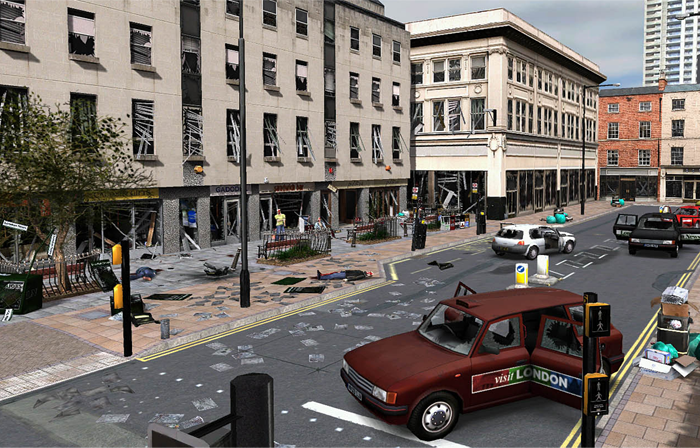
\includegraphics[scale=0.5]{tics/images/triage.png}
	\caption{Ambientación de Triage}
	\label{fig:triage}
\end{figure}

\emph{Visión General: } Triage Trainer se desarrolla en una escena de explosión
en una calle (ver~\ref{fig:triage}) la cual es un incidente mayor, y está
diseñado para formar profesionales que puedan participar en una escena de un
incidente de este tipo (médicos, enfermeros, paramédicos, rescatistas). Los
jugadores deben realizar un triaje, es decir, evaluar el grado de las lesiones
de víctima generadas aleatoriamente utilizando los protocolos y controles
médicos adecuados, además de priorizar a las víctimas para el tratamiento. La
apariencia física de cada víctima es imitada con precisión como los signos
vitales, los síntomas y sobre todo los patrones de tiempo para el deterioro de
las lesiones, es decir, la condición de una víctima cambia de forma realista con
el tiempo (ver~\ref{fig:triage_patient1}.

\begin{figure}[h!]
	\centering 
	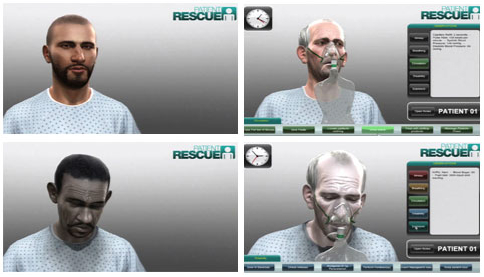
\includegraphics[scale=0.5]{tics/images/patient_side.jpg}
	\caption{Evolución de un paciente en Triage}
	\label{fig:triage_patient1}
\end{figure}

Los jugadores reciben retroalimentación acerca de su rendimiento, incluyendo la
precisión de sus chequeos, si los pacientes fueron priorizados en el orden
correcto y el tiempo que les llevó completar el triaje, en comparación con la de
un experto.

\emph{Evaluación: } La retroalimentación de los participantes que utilizaron
Triage Trainer sugiere que el mismo cumplió exitosamente sus fines. Los
jugadores asociaron su experiencia de juego con su experiencia en el mundo real
y muchos de ellos sentían que realmente estaban allí. Se espera que los
jugadores puedan tomar decisiones bajo presión, lo que ayudará a su desarrollo
cognitivo. También se observó que los jugadores tienden a discutir sus
experiencias con sus compañeros de curso, lo que también podría tener un impacto
en su aprendizaje.

Un elemento que no fue evaluado por TruSim debido a que no era logísticamente
posible fue el impacto de las pruebas en la retención del conocimiento y el
cambio de comportamiento de los jugadores~\cite{education:games}. 


\subsubsection{Caso 2 SimVenture}

\emph{Tipo: } Juego de simulación de negocios.

\emph{Destinatarios: } Personas de 14 a 30 años.

\emph{Contenido: } Las realidades de la creación y funcionamiento de un negocio.

\emph{Desarrollado por: } Venture Simulations.

\emph{Visión General: } En el inicio del
juego(ver~\ref{fig:simventure_tutorial}), a los jugadores se les brinda
informaciones y antecedentes para que que se ubiquen en escena. Ellos deben
empezar a dirigir su propio negocio en su casa de fabricación y venta de
computadoras, mientras deben mantener un trabajo de tiempo completo
independiente. El juego lleva a los jugadores a la ejecución de un negocio en su
propia casa a la extensión del mismo a más locales, lo que requiere contración
de personal. Los jugadores son capaces de avanzar en el juego a través del
aprendizaje de los elementos importantes del empresariado organizadas en cuatro
categorías: organización, ventas/marketing, finanzas y operaciones. Los
jugadores toman decisiones acerca de las actividades dentro de estas áreas y
observan los resultados de sus acciones. 

\begin{figure}[h!]
	\centering 
	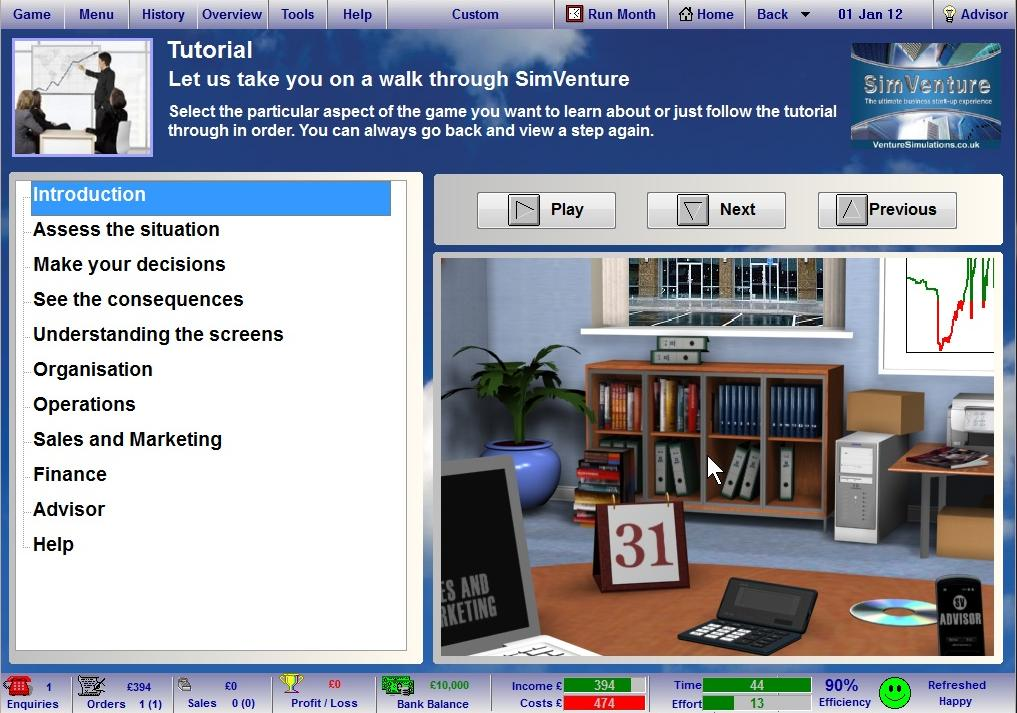
\includegraphics[scale=0.5]{tics/images/simventure-tutorial.jpg}
	\caption{Tutorial de SimVenture}
	\label{fig:simventure_tutorial}
\end{figure}

Los jugadores obtienen retroalimentación sobre un número de diferentes
parámetros. En un nivel básico, se puede simplemente revisar la cantidad de
ingresos que están generando. Además de esto, el éxito puede ser medido por la
cantidad de pedidos que han recibido para sus productos. También se proporciona
retroalimentación visual para representar la eficiencia de la organización y su
felicidad como individuo.

\emph{Evaluación: } Phil Warren, director de estudios de negocios en Snaith
School, ha utilizado SimVenture como complemento al plan de estudios. Según el
mismo, el plan de estudios por lo general sólo requiere que los estudiantes
aprender sobre los diversos elementos diferentes del negocio de forma aislada y
sin embargo, cualquier decisión que se tome en una de las partes de un negocio
tiene efecto en las demás. SimVenture se vió como una oportunidad de aplicar los
conocimientos aprendidos en clase en una actividad práctica, además se observó
que permitir que los estudiantes jueguen en pares da un espacio para la
discusión en torno a las decisiones y aprenden de sus errores
juntos~\cite{education:games}.

